% Appendix B (track hw). Circuits and rules behind Secs. 2.2 to 2.5: encoding circuit, action of
% the logical generators, check rounds of the two layouts (extraction circuits, gate moments,
% data-relay walk-through, single-fault check), noise channels and their placement, the three
% deviations from the reference models, fault budgets, qubit forms of the channels.
% Text moved from the main text of the 438f6f16 mirror (source lines in the comments) and revised;
% changes of content are listed in jpw-review/hw/content-changes.md, part G.
% In the circuit figures the gate labels with a dimension subscript (H_3, X_3, S_3, Z_3) were
% changed to plain symbols (CONTRACT Sec. 5, ruling 3); no circuit was redrawn.
\section{Check-Round Circuits and Noise Placement}
\label{app:rounds}
% TODO(sim): the text of this appendix still describes the seven-moment one-ancilla round, the single 4-gate encoder and the
% conventional-site two-ancilla layout; rewrite it in the appendix step of jpw-review/sim/restructure-plan.md (figures already new).

This appendix gives the circuits and rules behind \autoref{sub:code} to \autoref{sub:noise_models}: the encoding circuit and the action of the logical generators, the check rounds of the two layouts, the placement of the noise channels, and the fault budgets that follow from it.

\subsection{Encoding Circuit and Logical Generators}
\label{app:rounds-encoding}\label{app:rounds-conjugation}

% from "method - [[5,1,2]]_3 qutrit surface code.tex", lines 75-90
The encoding circuit of \autoref{fig:encoding_circuit} maps $\ket{0}^{\otimes 5}$ to $\ket{\bar{+}}$ with three one-qutrit and four two-qutrit gates and without ancillas. It is not fault tolerant. Because the encoding is noiseless in the simulations (\autoref{sub:noise_models}), it does not need to be.

\begin{figure*}[tp]
  % from paper-rework/a1-layout-figure/encoders-abc.pdf, caption-encoders.tex (restructure 2026-11-19)
  \centering
  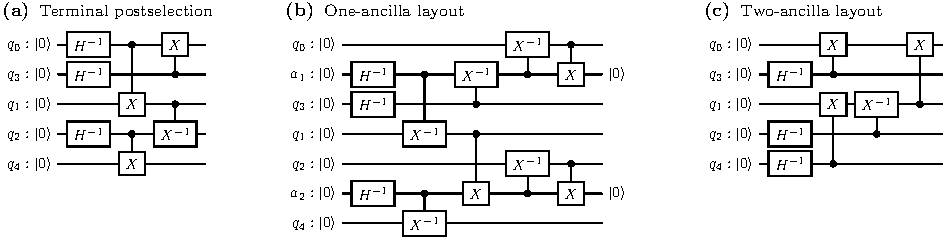
\includegraphics{figures/encoders-three.pdf}% drawn at final size
  \caption{Encoding circuits that prepare $q_0, \dots, q_4$ in $\ket{\bar{+}}$, the $+1$ eigenstate of $\bar X$ (Eq.~\eqref{eq:logicalPauli}), from $\ket{0}$ on every qutrit, in terminal postselection on IQM's Garnet QPU~\cite{IQM240812433} (a) and in the one-ancilla (b) and two-ancilla (c) layouts of \autoref{fig:ancilla_layouts}. Each circuit shows only the qutrits it acts on. $H^{-1}$ and SUM are the gates of Eq.~\eqref{eq:conventions}, and a dot connected to a box $X$ ($X^{-1}$) is a SUM gate (its inverse) with the control on the dot. Every two-qutrit gate acts on a coupling drawn in the matching panel of \autoref{fig:ancilla_layouts}. The rows are ordered so that each column holds one gate moment, a set of gates that act on disjoint qutrits and run in parallel. Counting the moment of the $H^{-1}$ gates, the circuits take three, five and four gate moments and have four, eight and four two-qutrit gates. Since the one-ancilla layout couples no two data qutrits other than $q_2$ and $q_3$, circuit (b) entangles the data through the ancillas $a_1$ and $a_2$, which end in $\ket{0}$. Because the simulations prepare $\ket{\bar{+}}$ without noise (\autoref{sub:noise_models}), their results do not depend on which circuit prepares it.}
  \label{fig:encoding_circuit}
\end{figure*}

% from "method - [[5,1,2]]_3 qutrit surface code.tex", lines 46-68. The table now names the generators; pairs checked by hand from Eqs. (eq:logical_H), (eq:logical_HS) and the rules of Eq. (eq:bg-conjugation).
\autoref{tab:clifford-conjugation} lists how the generators $\bar H$ and $\bar S$ of Eqs.~\eqref{eq:logical_H} and~\eqref{eq:logical_HS} conjugate the stabilizer generators and the logical Pauli operators. Both map the stabilizer group to itself, and they act on $\bar X$ and $\bar Z$ as $H$ and $S$ act on $X$ and $Z$ in Eq.~\eqref{eq:bg-conjugation}.

\begin{table*}[tp]
  \centering
  \begin{tabular}{l|l}
    \hline
    Stabilizer generators & Logical Paulis \\
    \hline
    $\bar H G_1 \bar H^\dagger = G_3^{-1}$, \quad $\bar H G_2 \bar H^\dagger = G_4^{-1}$
      & $\bar H \bar Z \bar H^\dagger = \bar X^{-1}$ \\
    $\bar H G_3 \bar H^\dagger = G_1$, \quad $\bar H G_4 \bar H^\dagger = G_2$
      & $\bar H \bar X \bar H^\dagger = \bar Z$ \\
    $\bar S G_1 \bar S^\dagger = G_1$, \quad $\bar S G_2 \bar S^\dagger = G_2$
      & $\bar S \bar Z \bar S^\dagger = \bar Z$ \\
    $\bar S G_3 \bar S^\dagger = G_3 G_1$, \quad $\bar S G_4 \bar S^\dagger = G_4 G_2$
      & $\bar S \bar X \bar S^\dagger = \bar X \bar Z$ \\
    \hline
  \end{tabular}
  \caption{Conjugation of the stabilizer generators $G_1, \dots, G_4$ (left) and of the logical Pauli operators (right) of the $[[5,1,2]]_3$ code by the logical Clifford generators $\bar H$ and $\bar S$.}
  \label{tab:clifford-conjugation}
\end{table*}

\subsection{Check Round of the One-Ancilla Layout}
\label{app:rounds-one-ancilla}

% from "method - LRB-D.tex", lines 179 (text) and 96-149 (panels (c), (d) of the former protocol figure)
In the one-ancilla layout the ancilla $a_j$ measures $G_j$ with the circuits of \autoref{fig:rounds_one_ancilla}. For the $Z$-type stabilizers $G_1$ and $G_2$, each of the three data qutrits controls a SUM gate or its inverse onto the ancilla, which collects the syndrome in the computational basis. For the $X$-type stabilizers $G_3$ and $G_4$, the ancilla is rotated by $H$, controls a SUM gate or its inverse onto each of the three data qutrits, and is rotated back by $H^{-1}$ before its computational-basis readout. A data qutrit that enters a stabilizer with the exponent $-1$ takes the inverse SUM gate. The round uses all 12 couplings between a site and a neighboring data qutrit, and \autoref{tab:conv_round} lists its gate moments.

\begin{figure*}[tp]
  % from paper-rework/a1-layout-figure/checks-bc.pdf (one-ancilla panels: the five-moment round), caption-checks-bc.tex (restructure 2026-11-19)
  \centering
  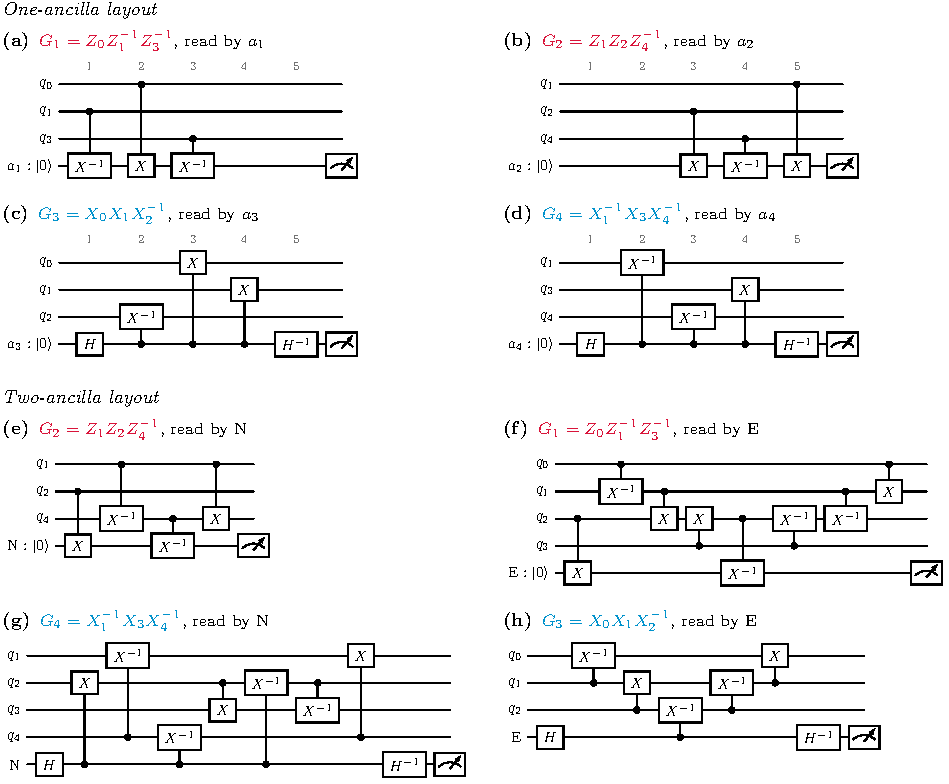
\includegraphics{figures/extraction-two-layouts.pdf}% drawn at final size
  \caption{Syndrome extraction circuits of the two layouts of \autoref{fig:ancilla_layouts}: the one-ancilla layout in (a)--(d) and the two-ancilla layout, with the ancillas N and E, in (e)--(h). Each panel shows only the qutrits it acts on. In (a)--(d) the numbered columns are the gate moments of the round, the time steps in which gates on disjoint qutrits run in parallel, and in (e)--(h) the gates appear in the order in which the round's circuit lists them. The gates are those of Eq.~\eqref{eq:conventions}. A dot connected to a box $X$ ($X^{-1}$) is a SUM gate (its inverse) with the control on the dot, and $\mathrm{SUM}(q_4 \to q_1)$, for example, adds the computational-basis value of the control $q_4$ to the target $q_1$. A data gate is a SUM gate or its inverse between two data qutrits. Let $z_j$ be the computational-basis value of $q_j$, and let the syndrome of $G_j$ be the exponent of $\omega = e^{2\pi i/3}$ in its eigenvalue.
(a)--(d)~Ancilla $a_j$ measures $G_j$ without data gates, with one SUM gate or its inverse per data qutrit of $G_j$, between $H$ and $H^{-1}$ for the $X$-type $G_3$ and $G_4$. The four ancillas are reset to $\ket{0}$ at the start of each check round and read out together at its end. The round runs its 12 two-qutrit and four one-qutrit gates in five gate moments, and an ancilla idles in a moment whose column holds no gate.
(e)--(h)~Panels (e) and (f) form the first half of the round and (g) and (h) the second, with 24 two-qutrit and four one-qutrit gates in all. N and E are reset to $\ket{0}$ at the start of the round, read out at the end of each half and not reset between the halves.
(e)~N adds $z_2$, a data gate sets $q_4$ to $z_4 - z_1$, N subtracts this value, and the data gate is undone, so N holds $z_1 + z_2 - z_4$, the syndrome of $G_2$.
(f)~E adds $z_2$, data gates add $z_1 - z_0 + z_3$ to $q_2$, E subtracts the new value of $q_2$, and the data gates are undone, so E holds $z_0 - z_1 - z_3$, the syndrome of $G_1$.
(g), (h)~Between $H$ and $H^{-1}$ the ancilla controls SUM gates or their inverses onto the data and so collects the eigenvalue of an $X$-type operator. We write each such operator as it acts on the data before the first data gate. In (g), N collects $X_2$ through $q_2$, then $X_1^{-1} X_4^{-1}$ through $q_4$ while $\mathrm{SUM}^{-1}(q_4 \to q_1)$ is in place, and then $X_2^{-1} X_3$ through $q_2$ while $\mathrm{SUM}(q_2 \to q_3)$ is also in place. Their product is $G_4$. In (h), E collects $G_3$ through $q_2$, its only neighbor, while $\mathrm{SUM}^{-1}(q_1 \to q_0)$ and $\mathrm{SUM}(q_2 \to q_1)$ are in place. The data gates are undone before the readout. Because N and E are not reset, the second readout of N is its first readout plus the syndrome of $G_4$, and that of E its first readout plus the syndrome of $G_3$, modulo three.}
  \label{fig:extraction_circuits}\label{fig:rounds_one_ancilla}
\end{figure*}

\subsection{Check Round of the Two-Ancilla Layout}
\label{app:rounds-relay}

% from "method - LRB-D.tex", lines 181-183
In the two-ancilla layout we call the four sites N, W, E and S (\autoref{fig:ancilla_layouts}(c)). N is next to $q_0$, $q_1$ and $q_2$, W to $q_0$, $q_2$ and $q_3$, E to $q_1$, $q_2$ and $q_4$, and S to $q_2$, $q_3$ and $q_4$, so that N can measure $G_3$ and E can measure $G_2$. Another choice of generators would not remove the need for two sites, because the elements of the stabilizer group that could replace $G_1$ or $G_4$ have weight four or five. Nor can the two parts of a boundary stabilizer be read on separate sites and added afterward, because reading a site measures the operator that the site has collected on the data. If N collected $Z_0 Z_1^{-1}$ and E collected $X_1^{-1} X_4^{-1}$, for example, W would read $Z_3^{-1}$ and S would read $X_3$. Every round would then measure $q_3$ in the $Z$ basis and in the $X$ basis, and each of the two readouts would randomize the other.

% from "method - LRB-D.tex", line 183
The data relay instead moves a partial value through a data qutrit, so that one site holds the whole stabilizer before any site is read (\autoref{tab:conv_round}). Let $z_j$ be the computational-basis value of $q_j$, so that the syndrome of $G_1$ is $z_0 - z_1 - z_3$ modulo three. N first measures $G_3$. It then collects $-z_1$ and lends its value to $q_0$ with a SUM gate, which adds this value to that of $q_0$. W collects the value of $q_0$ and $-z_3$. N then takes its value back from $q_0$ and clears the $-z_1$ part against $q_1$. Because N still holds the syndrome of $G_3$ while it lends, W ends with the syndrome of $G_1$ shifted by that of $G_3$. $G_4$ is measured in the same way in the $X$ basis: E collects the part on $q_1$ and lends it to $q_4$, S collects the parts on $q_4$ and $q_3$, and E takes its value back before it measures $G_2$. At the end of the round N holds the syndrome of $G_3$, W that of $G_1$ shifted by the value of N, E that of $G_2$ and S that of $G_4$, each up to a sign. All four readouts are zero exactly when all four syndromes are trivial, so the acceptance rule of \autoref{sub:lrb_d} applies to the readouts unchanged. The round uses 10 of the 12 couplings between a site and a neighboring data qutrit, because W and S never act on $q_2$. As in the one-ancilla round, every two-qutrit gate acts on one ancilla and one data qutrit.

% Moments as scheduled by the production generator: FoldedQutritDetectionCode and FoldedQutritConventionalSitesDetectionCode.conventional_sites_check_round_circuit (conventional-sites worktree, src/lrb/code_definitions.py), scheduled with LRBCircuitGenerator.schedule_moments in paper-rework/scratch/writer-conv/budget.py (budget.out). The column of the one-ancilla round is new (same source).
\begin{table*}[tp]
  \centering
  \footnotesize
  \setlength{\tabcolsep}{4pt}
  \begin{tabular}{c|l|l}
    \hline
    Moment & One-ancilla round & Two-ancilla round \\
    \hline
    1 & $\mathrm{SUM}(q_0 \to a_1)$, $H$ on $a_3$, $a_4$ & $H$ on E, S, N \\
    2 & $\mathrm{SUM}^{-1}(q_1 \to a_1)$, $\mathrm{SUM}(a_3 \to q_0)$ & $\mathrm{SUM}(\mathrm{E} \to q_1)$, $\mathrm{SUM}^{-1}(\mathrm{S} \to q_3)$, $\mathrm{SUM}(\mathrm{N} \to q_0)$ \\
    3 & $\mathrm{SUM}^{-1}(q_3 \to a_1)$, $\mathrm{SUM}(q_1 \to a_2)$ & $\mathrm{SUM}(q_4 \to \mathrm{E})$, $\mathrm{SUM}^{-1}(q_3 \to \mathrm{W})$, $\mathrm{SUM}^{-1}(\mathrm{N} \to q_2)$ \\
    4 & $\mathrm{SUM}(q_2 \to a_2)$, $\mathrm{SUM}(a_3 \to q_1)$, $\mathrm{SUM}(a_4 \to q_3)$ & $\mathrm{SUM}(\mathrm{S} \to q_4)$, $\mathrm{SUM}(\mathrm{N} \to q_1)$ \\
    5 & $\mathrm{SUM}^{-1}(q_4 \to a_2)$, $\mathrm{SUM}^{-1}(a_3 \to q_2)$, $\mathrm{SUM}^{-1}(a_4 \to q_1)$ & $H^{-1}$ on S, N, $\mathrm{SUM}^{-1}(q_4 \to \mathrm{E})$ \\
    6 & $H^{-1}$ on $a_3$, $\mathrm{SUM}^{-1}(a_4 \to q_4)$ & $\mathrm{SUM}^{-1}(\mathrm{E} \to q_1)$ \\
    7 & $H^{-1}$ on $a_4$ & $\mathrm{SUM}^{-1}(q_1 \to \mathrm{N})$, $H^{-1}$ on E \\
    8 & & $\mathrm{SUM}(\mathrm{N} \to q_0)$, $\mathrm{SUM}(q_2 \to \mathrm{E})$ \\
    9 & & $\mathrm{SUM}^{-1}(q_4 \to \mathrm{E})$, $\mathrm{SUM}(q_0 \to \mathrm{W})$ \\
    10 & & $\mathrm{SUM}^{-1}(\mathrm{N} \to q_0)$, $\mathrm{SUM}(q_1 \to \mathrm{E})$ \\
    11 & & $\mathrm{SUM}(q_1 \to \mathrm{N})$ \\
    \hline
  \end{tabular}
  \caption{Gate moments of one check round in the two layouts, as scheduled in the simulations. Each round starts with one moment that resets its four ancillas and ends with one moment that reads them out. $\mathrm{SUM}(a \to b)$ adds the computational-basis value of $a$ to $b$, and $\mathrm{SUM}^{-1}(a \to b)$ subtracts it. For a site in the $X$ basis, between its $H$ and its $H^{-1}$, $\mathrm{SUM}(a \to b)$ instead subtracts the $X$-basis value of $b$ from that of $a$, so that $X$-basis values move against the arrow. In the two-ancilla round, N measures $G_3$ and S measures $G_4$ in moments 1 to 5, while E collects the part on $q_1$, lends it to $q_4$ in moment 3 and takes it back in moment 5. E clears itself against $q_1$ in moment 6 and measures $G_2$ in moments 8 to 10. N collects $-z_1$ in moment 7, lends its value to $q_0$ in moment 8, takes it back in moment 10 and clears itself against $q_1$ in moment 11. W collects $-z_3$ in moment 3 and the value of $q_0$ in moment 9.}
  \label{tab:conv_round}
\end{table*}

% Single-fault enumeration of the two simulated rounds, as the production generator builds them: jpw-review/hw/checks/check_single_faults.py (.out), written by the technical verifier of critic round 1: 1400 and 2072 faults of the noise-model channels, none missed by both rounds and logical; a superset (every one-qutrit Pauli on every wire after every operation, every two-qutrit Pauli after every two-qutrit gate; 2760 and 3816 faults) gives the same result; qubit rounds: 347 and 509 faults, none. The earlier record (LRB-experiment-data-slurm/comparisons/two-ancilla-checks/fault_check.py and CONV-SITES-FACTS.md) covers the one-ancilla round and earlier relay schedules.
\paragraph{Single faults.} We checked by enumeration that neither round lets a single fault through. One Pauli fault is placed in the first of two otherwise noiseless rounds. The fault set contains every channel that the noise models place in a round, at every location and with every Pauli of that channel, which gives $1400$ faults in the one-ancilla round and $2072$ in the two-ancilla round. A fault counts as an undetected logical error if every ancilla readout of both rounds is zero while the error that remains on the data qutrits is a logical operator. The fault set contains no undetected logical error in either layout.

\subsection{Noise Channels and Their Placement}
\label{app:rounds-noise}\label{app:rounds-protocol}

% from "noise models.tex", lines 8-22
The three channels of \autoref{sub:noise_models} act on a state $\rho$ as
\begin{align}
    \mathrm{DEP1}(p)\colon\quad \rho &\mapsto (1-p)\,\rho + \frac{p}{8}\sum_{P \neq I} P \rho\, P^\dagger , \\
    \mathrm{DEP2}(p)\colon\quad \rho &\mapsto (1-p)\,\rho + \frac{p}{80}\sum_{P \neq I \otimes I} P \rho\, P^\dagger ,
    \label{eq:2-depol} \\
    \mathrm{flip}(p)\colon\quad \rho &\mapsto (1-p)\,\rho + \frac{p}{2}\left( X \rho X^\dagger + X^2 \rho\, (X^2)^\dagger \right) ,
    \label{eq:flip-channel}
\end{align}
where $P$ runs over the non-identity Paulis $X^a Z^b$ of one qutrit and over their $80$ non-identity products on two qutrits. The argument is the probability that the channel applies a non-identity Pauli, and every rate of \autoref{tab:circuit-noise} is such a probability. DEP1 is the depolarizing channel of Eq.~\eqref{eq:1-depol} with $p_{\mathrm{mix}} = \tfrac{9}{8}\,p$, because one ninth of the uniform mixture over all nine Paulis reproduces the input state, and DEP2 is the two-qutrit channel $(1-p_{\mathrm{mix}})\,\rho + \tfrac{p_{\mathrm{mix}}}{9} I$ with $p_{\mathrm{mix}} = \tfrac{81}{80}\,p$. The names DEP1 and DEP2 follow~\cite{GidneyHoneycomb2021}, whose classical bit flips on resets and measurements become the flip channel for qutrits. A shift $X^a$ with $a \neq 0$ immediately before a computational-basis measurement changes the recorded outcome by $a$ modulo three.

% from "noise models.tex", lines 26-28, and "method - LRB-D.tex", lines 18 and 22
The channels are placed after the circuit is divided into segments. Each logical Clifford, each check round and each Clifford of the baseline is one segment. Within a segment every gate goes into the earliest moment after the previous operation on each of its qutrits, so that operations on disjoint qutrits run in parallel and the order on each qutrit is kept. A moment holds either gates or resets and measurements, never both. Measurements whose qutrit is not used again in the segment are moved to one final moment, so that all ancilla readouts of a check round share its last moment. An ancilla whose extraction circuit ends earlier idles until then, which accounts for 7 of the 35 idle locations in the gate moments of the one-ancilla round and for 9 of the 57 of the two-ancilla round. No moment spans two segments. The identity element of the Clifford group is applied as an identity gate that occupies one moment and receives the idle noise of a gate moment.

% from "noise models.tex", lines 28 and 50, and the caption of the former table
Every moment then receives the channels of \autoref{tab:circuit-noise} (\autoref{fig:lrb_b} shows an example). The full models contain two further rules, which have no effect in our circuits. The first puts a phase flip, the channel of Eq.~\eqref{eq:flip-channel} with $Z$ and $Z^2$ in place of $X$ and $X^2$, before each $X$-basis measurement, with probability $5p$ under SI1000 and $p$ under SD6. It never applies, because every readout of our circuits is a computational-basis measurement: the $X$-type extraction circuits rotate their ancillas with $H^{-1}$ before the readout. The second puts DEP1 with probability $p$ after each measurement under both models. It acts only on ancillas that are reset before their next use or are not used again, so it changes no detector and no logical outcome. SI1000 requires $p \le 0.2$, so that the probability $5p$ of a measurement flip is at most one.

% from "method - LRB-D.tex", lines 80-94: panel (b) of the former protocol figure, with the matching part of its caption
\begin{figure*}[tp]
    \centering
    \scalebox{0.8}{
    \begin{quantikz}[row sep={0.75cm,between origins}, column sep=0.25cm]
      \lstick{$q_0$} & \gate{S} & \gate{\textcolor{purple}{\mathcal{E}_1}} & \qw \\
      \lstick{$q_1$} & \gate{S^{-1}} & \gate{\textcolor{purple}{\mathcal{E}_1}} & \qw \\
      \lstick{$q_2$} & \ctrl{1} & \gate[2]{\textcolor{purple}{\mathcal{E}_2}} & \qw \\
      \lstick{$q_3$} & \gate{Z} & & \qw \\
      \lstick{$q_4$} & \gate{S} & \gate{\textcolor{purple}{\mathcal{E}_1}} & \qw \\
      \lstick{ancillas} & \qwbundle{n_a} & \gate{\textcolor{purple}{\mathcal{E}_{\mathrm{idle}}}} & \qw
    \end{quantikz}
    }
    \caption{Noise in one segment, here a logical Clifford that consists of $\bar S$ alone and occupies one moment. $\mathcal{E}_1$ is DEP1 after a one-qutrit gate, $\mathcal{E}_2$ is DEP2 after the CZ gate on $q_2$ and $q_3$, and $\mathcal{E}_{\mathrm{idle}}$ is the idle DEP1 on each of the $n_a = 4$ ancillas. $\mathcal{E}_1$ and $\mathcal{E}_{\mathrm{idle}}$ have probability $p/10$ under SI1000 and $p$ under SD6, and $\mathcal{E}_2$ has probability $p$.}
    \label{fig:lrb_b}\label{fig:rounds_segment_noise}
\end{figure*}

\subsection{Deviations from the Reference Models}
\label{app:rounds-deviations}

% from "noise models.tex", lines 52-55
% TODO(authors): confirm that these deviations from the reference noise models are intended (native SUM, CZ and SWAP under both models, no stacking of Idle(p/10) and ResonatorIdle(2p) under SI1000, post-measurement DEP1 in both models).
Our models deviate from those of~\cite{GidneyHoneycomb2021} in three points. First, they contain DEP1 after every measurement, a rule that the reference models lack and that has no effect in our circuits (\appref{app:rounds-noise}). Second, under SI1000 a qutrit that idles in a reset or measurement moment receives DEP1 with probability $2p$ only, whereas in the reference model the rules Idle($p/10$) and ResonatorIdle($2p$) both act on such a qubit. Third, SUM, CZ, their inverses and SWAP are each one native two-qutrit gate followed by DEP2. The reference gate sets contain a single entangling gate, CZ for SI1000 and CNOT for SD6, so that a SWAP or an entangling gate of the other type would there be compiled into several entangling and one-qubit gates.

\subsection{Fault Budgets}
\label{app:rounds-budget}

% Location counts and budgets: paper-rework/scratch/writer-conv/budget.py (budget.out) and jpw-review/hw/checks/check_fault_budgets.py (.out), from the generator of the conventional-sites worktree. Sums: 12 + 0.4 + 8 + 20 + 4 + 3.5 + 20 = 67.9; 18 + 0.6 + 8 + 20 + 4 + 5.7 + 20 = 76.3; 12 + 4 + 4 + 4 + 4 + 35 + 10 = 73; 18 + 6 + 4 + 4 + 4 + 57 + 10 = 103. Logical Clifford: mean over the 216 catalog words, data wires only, 5.73p (SI1000) and 28.78p (SD6); the inverse words give the same means.
\begin{table*}[tp]
  \centering
  \begin{tabular}{l|c|c|c|c|c}
    \hline
    & & \multicolumn{2}{c|}{Locations} & \multicolumn{2}{c}{Probability} \\
    Location & Channel & one-anc. & two-anc. & SI1000 & SD6 \\
    \hline
    Two-qutrit gate & DEP2 & 12 & 18 & $p$ & $p$ \\
    One-qutrit gate & DEP1 & 4 & 6 & $p/10$ & $p$ \\
    Reset & flip & 4 & 4 & $2p$ & $p$ \\
    Measurement, before & flip & 4 & 4 & $5p$ & $p$ \\
    Measurement, after & DEP1 & 4 & 4 & $p$ & $p$ \\
    Idle qutrit in a gate moment & DEP1 & 35 & 57 & $p/10$ & $p$ \\
    Idle qutrit in a reset or measurement moment & DEP1 & 10 & 10 & $2p$ & $p$ \\
    \hline
    Expected number of faults, one-ancilla round & & & & $67.9p$ & $73p$ \\
    Expected number of faults, two-ancilla round & & & & $76.3p$ & $103p$ \\
    \hline
  \end{tabular}
  \caption{Noise locations of one check round in the one-ancilla and in the two-ancilla layout, with the probability of each channel under SI1000 and SD6. The expected number of faults of a round is the sum of the probabilities over its locations.}
  \label{tab:round-budget}
\end{table*}

\autoref{tab:round-budget} derives the expected number of faults of a check round from its noise locations. The count includes the $4p$ of DEP1 after the measurements, which change no detector. The flips on resets and measurements contribute $28p$ of the budget of either round under SI1000 and $8p$ under SD6. The data relay adds $8.4p$ under SI1000, of which $6p$ come from its six two-qutrit gates, $2.2p$ from the 22 idle locations of its four gate moments and $0.2p$ from its two one-qutrit gates. Under SD6 it adds $30p$, of which the same idle locations contribute $22p$.

For a logical Clifford we count the channels on the data qutrits and average over the $216$ words of \appref{sec:clifford-gen}, which gives $5.73p$ under SI1000 and $28.8p$ under SD6. The count leaves out the idle DEP1 on the ancillas during a logical Clifford, because the reset at the start of the next check round erases its effect. One unit of depth holds two logical Cliffords and one check round. Its two Cliffords thus carry $11.5p$ against the $67.9p$ of the one-ancilla round under SI1000, and $57.6p$ against $73p$ under SD6.

\subsection{Qubit Forms of the Channels}
\label{app:rounds-qubit}

% from "method.tex", lines 18-19
% Qubit noise channels: sdim 1.4.0 (N1 'd' uniform over the q^2 - 1 non-identity Paulis, N1 'f'/'p' over the q - 1 nonzero shifts, N2 uniform over the q^4 - 1 non-identity Paulis) and CIRCUIT_LEVEL_NOISE_RATES in src/lrb/circuit_generator.py, identical in the qubit-lrbd-sdim140 and conventional-sites worktrees; mixing forms checked in paper-rework/scratch/corrector-qubit-1/corrector.py (section H)
For the qubit code of \autoref{sub:qubit_code}, DEP1 with probability $p$ applies each of $X$, $Z$ and $XZ$ with probability $p/3$, which is the depolarizing channel with $p_{\mathrm{mix}} = \tfrac{4}{3}\,p$, and DEP2 applies each of the $15$ non-identity two-qubit Paulis with probability $p/15$, which corresponds to $p_{\mathrm{mix}} = \tfrac{16}{15}\,p$. A flip with probability $p$ applies $X$ and inverts the recorded bit. These are the channels of~\cite{GidneyHoneycomb2021} themselves, so the qubit models are the reference models up to the three deviations of \appref{app:rounds-deviations}, with CNOT in place of SUM. The check rounds, their scheduling and the location counts of \autoref{tab:round-budget} are the same as for the qutrit code, and the single-fault enumeration finds no undetected logical error among the $347$ and $509$ faults of the two qubit rounds. A logical Clifford of the qubit code puts $2.80p$ on the data qubits under SI1000 and $14.5p$ under SD6.
